

% ***************************************************
% Arranged by: Abdul Waris Ayazi
% Date : 2026 - March - 11
% Kabul University
% ***************************************************


\documentclass[instructions]{StylesAndSettings/uqthesis}
%\documentclass[final]{StylesAndSettings/uqthesis} 


\setlength{\footskip}{9mm}

\input{dsfont.sty}

\input{StylesAndSettings/LaTexPackages.tex}

% ***************************************************
% Title page
% ***************************************************

%***THESIS TITLE***
%Use Sentence Case (capitalise only the first word and proper nouns).
\title{Sign Language }

%***YOUR NAME***
%Do not include initials or middle names.
\author{Waris Mustafa}


%***Full Name of supervisor***
\supervisor{Dr. Nesar Ahmad Wasi}

%***YEAR OF SUBMISSION***
\date{May 2026}


%HBAR fix added by Michael
% (this issue is related to the use of the mathptmx package)
\begin{document}
\renewcommand{\hbar}{\mathchar'26\mkern-7.5mu h}


\frontmatter

% Assemble title page
\maketitle
\clearpage
\setcounter{page}{1}


% Preface
%****************************************************
\pagestyle{plain}
\newpage
\null
\newpage
\begin{figure}[t!] 
	\begin{center}
		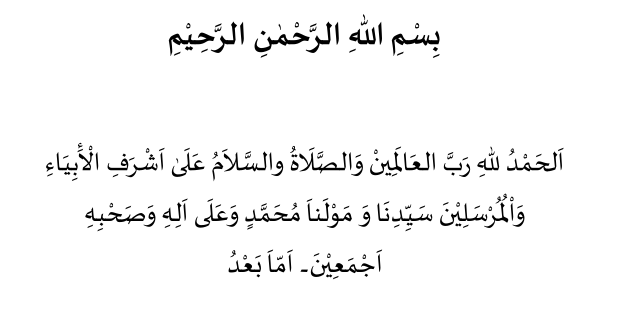
\includegraphics[width=1.0\linewidth]{Resources/start}
	\end{center}
	\label{fig:resnet}
\end{figure}
\clearpage
\pagestyle{plain}


\newpage
\null
\newpage
% ***************************************************
% Certificate of Approval 
% ***************************************************


\section{Certificate of Approval}
We certify that we have read the “PROJECT NAME” report
submitted by (SOMEONE 1) and (SOMEONE 2) as partial fulfillment
for the award of the degree of Bachelor of Information Technology
Faculty of Computer Science at Kabul University. We have evaluated
the report and found it up to the requirements in its scope and quality
for the award of the degree.\\

\begin{adjustwidth}{1in}{}
	\Large
	Supervisor Name: \\
	Signature:\_\_\_\_\_\_\_\_\_\_\_\_\_\_\_\_\_\_\_\_\_\_\_\_\_\_\_\_\_\_\_\_ \\
	Date :\_\_\_\_\_\_\_\_\_\_\_\_\_\_\_\_\_\_\_\_\_\_\_\_\_\_\_\_\_\_\_\\ 
	
	
	Name: \\
	(Head of Information Systems Department) \\
	Signature:\_\_\_\_\_\_\_\_\_\_\_\_\_\_\_\_\_\_\_\_\_\_\_\_\_\_\_\_\_\_\_\\
	Date :\_\_\_\_\_\_\_\_\_\_\_\_\_\_\_\_\_\_\_\_\_\_\_\_\_\_\_\_\_\_\_\\ 
	
	
	Name: \\
	(Dean of Computer Science Faculty) \\
	Signature:\_\_\_\_\_\_\_\_\_\_\_\_\_\_\_\_\_\_\_\_\_\_\_\_\_\_\_\_\_\_\_\\\
	Date :\_\_\_\_\_\_\_\_\_\_\_\_\_\_\_\_\_\_\_\_\_\_\_\_\_\_\_\_\_\_\_
	
	
\end{adjustwidth}


\clearpage
\pagestyle{plain}
% ***************************************************
% Author's Declaration
% ***************************************************
\newpage
\null
\newpage

\section{Author's Declaration}
Hereby I, xxxxx, declare that this Bachelor thesis is my personal
achievement and the result of an original investigation. I further state
that this thesis has not been previously submitted for any other
academic degree.\\


\begin{center}
	\text Date: April-2025
\end{center}

\vspace{30 pt}

\begin{flushleft}
Student ID: \\
Student Name and Sign:\_\_\_\_\_\_\_\_\_\_\_\_\_\_\_\_\_\_\_\_\_\_\_\_\_\_\_\_\_\_\_\	
\end{flushleft}

\newpage
\null
\newpage


\clearpage
\pagestyle{plain}
\section*{Abstract}
\normalfont

%Open abstract.tex to edit

% ***************************************************
% Abstract
% ***************************************************

\begin{instructional}
	Start this section on a new page [this template will automatically handle this]. \\
	Your paragraphs go here. Your paragraphs line spacing should be
	1.15pt. Your paragraphs go here. Your paragraphs line spacing should
	be 1.15. Your paragraphs should be indented.\\
	\cite(Cawvey2017) \\
	\textbf{keywords:} keyword 1, …, keyword 7 (should be between 4 to 7)\\
	
	\\
	
	
	
	Important Notes:
	\begin{itemize}
		\item The main content should be more than 10,000 words
		\item All titles should be written with (Bahij Titr, Bold) font
		\item Normal text can be written with either (Bahij zar, B mitra, B zar, B Nazanin) font faces
		\item Font size for normal text is 12 with line spacing 0.1
		\item Tables titles should be 12 with (B mitra, B zar, B Nazanin) font faces
		\item ables contents should be 10 with (B mitra, B zar, B Nazanin) font face
		\item Figure description should be 10 with (B mitra,
		B zar, B Nazanin) font faces located under the figure
	\end{itemize}
	
	
\end{instructional}
\newpage
\null
\newpage



\clearpage



%***Acknowledgements***

\section*{Acknowledgments}

\begin{instructional}
    Start this section on a new page [the template will handle this for you].\\
    
    \noindent
    This is a free text section for you to record your gratitude to those who provided academic input and support and non-academic support during your candidature.
\end{instructional}


\newpage
\null
\newpage
%***Table of Contents***
%These generate the table of contents, list of figures, and list of tables from items tagged with a \label{} command.
\tableofcontents*
	\clearpage
\listoffigures
	\clearpage
\listoftables


%*************************************
% List of abbreviations
%*************************************
% You can make a list of abbreviations here. REMOVE IF NOT NEEDED.
%
% There are LaTeX packages available to take care of these things, but you will
% need to manually add these to the template at this stage (support may be added
% in future releases).

%CHOOSE AN APPROPRIATE TITLE.
%\chapter[List of abbreviations]{List of abbreviations}
\chapter[List of Abbreviations and Symbols]{List of Abbreviations and Symbols}

%If the auto-sizing of the tables annoys you, consider the tabularx package.
keywords
\begin{itemize}
	 
	\item It should be relevant to the title and overall purpose of the article and should be selected from the same categories.
	\item Select a word that is repeated several times in the text.
	\item Do not try to choose a compound word.
	\item Be related to the topic title.
	\item The minimum number of keywords should be 4 and the maximum should be 7 words.
\end{itemize}

%List of abbreviations.
\section{Abbreviations}



\noindent
\begin{longtable}{p{0.10\linewidth} p{0.80\linewidth} }
	AC & Alternating Current \\
	AFM	& Atomic Force Microscopy/Microscope \\
	\etc{} & \etc{} \\
\end{longtable}


%*************************************
% List of symbols
%*************************************
%List of symbols. REMOVE IF NOT NEEDED.
\section{Symbols}
\noindent
\begin{longtable}{p{0.10\linewidth} p{0.80\linewidth} }
	$\hat{\rho}$ & Density operator \\
	\etc{} & \etc{} \\
\end{longtable}
\clearpage

%***End of list of symbols and abbreviations***




%***End of front matter***
\clearpage


% ***************************************************
% Header and Foote
%****************************************************
\pagestyle{fancy}
% Clear default header/footer
\fancyhf{}

% Even pages (left side): Chapter title
\fancyhead[LE]{\nouppercase{\leftmark}}

% Odd pages (right side): Section title
\fancyhead[RO]{\nouppercase{\rightmark}}

% Page number at footer center
\fancyfoot[C]{\thepage}

\renewcommand{\chaptermark}[1]{%
	\markboth{#1}{}}

\renewcommand{\sectionmark}[1]{%
	\markright{\thesection\ #1}}




%YOU MUST EDIT THIS DOCUMENT.

% ***************************************************
% Thesis Content
%****************************************************

\mainmatter
%Each chapter is a separate .tex file. Use \input to load them here, as demonstrated below for Chapter 1 and Chapter 2.
%We recommend keeping each in a separate subfolder, with its accompanying figures, etc. This is how the template is currently structured.
%If you wish to divide your thesis into parts (each containing multiple chapters), us the \part{} command.



%CHAPTER 1
\chapter[Introduction]{Introduction}
\label{Chap:Intro}
\counterwithout{table}{chapter} % This ensures table numbering doesn't include the Chapter number through the document
\counterwithout{figure}{chapter}

\makeatletter
\setlength{\@fptop}{0pt} % This sets figures to the top of a page
\makeatother

% ***************************************************
% Introduction
% ***************************************************

% ********* Enter your text below this line: ********
\section{What is Sign language?}
Sign languages (also known as signed language) are languages that use the visual gestural modality to convey meaning through manual articulations in combination with
non-manual elements like the face and body. Afghan Sign Language (ASL)
is not a visual form of Afghani languages(Pashto or Dari) but its own unique language.
Sign Language Processing is an emerging field of
artificial intelligence concerned with the automatic processing and analysis of sign
language content. While research has focused more on the visual aspects of signed
languages, it is a subfield of both Natural Language Processing (NLP) and Computer
Vision (CV).

Challenges in sign language processing often include machine translation of
sign language videos into spoken language text (sign language translation), from spoken
language text (sign language production), or sign language recognition for sign language
understanding.



(Brief) History of Signed Languages and Deaf Culture

Throughout modern history, spoken languages were dominant, so much so that signed
languages struggled to be recognized as languages in their own right, and educators
developed misconceptions that signed language acquisition might hinder the
development of speech skills. For example, in 1880, a large international conference of
deaf educators called the “Second International Congress on Education of the Deaf”
banned teaching signed languages, favoring speech therapy instead. It was not until the
seminal work on American Sign Language (ASL) by Stokoe Jr (1960) that signed languages
started gaining recognition as natural, independent, and well-defined languages, which
inspired other researchers to further explore signed languages as a research area.
Nevertheless, antiquated attitudes that placed less importance on signed languagescontinue to inflict harm and subject many to linguistic neglect (Humphries et al. 2016).
Several studies have shown that deaf children raised solely with spoken languages do not
gain enough access to a first language during their critical period of language
acquisition (Murray, Hall, and Snoddon 2020). This language deprivation can lead to life-
long consequences on the cognitive, linguistic, socio-emotional, and academic
development of the deaf (Hall, Levin, and Anderson 2017).
Signed languages are the primary languages of communication for the Deaf1 and are at
the heart of Deaf communities. In the past, the failure to recognize signed languages as
fully-fledged natural language systems in their own right has had detrimental effects, and
in an increasingly digitized world, NLP research should strive to enable a world in which
all people, including the Deaf, have access to languages that fit their lived experience.
Sign Language Linguistics Overview
Signed languages consist of phonological, morphological, syntactic, and semantic levels
of structure that fulfill the same social, cognitive, and communicative purposes as other
natural languages. While spoken languages primarily channel the oral-auditory modality,
signed languages use the visual-gestural modality, relying on the signer’s face, hands,
body, and space around them to create distinctions in meaning. We present the linguistic
features of signed languages2 that researchers must consider during their modeling.
Phonology
Signs are composed of minimal units that combine manual features such as hand configuration,
palm orientation, placement, contact, path movement, local movement, as well as non-manual
features including eye aperture, head movement, and torso positioning (Liddell and Johnson 1989;
Johnson and Liddell 2011; Brentari 2011; Sandler 2012). Not all possible phonemes are realized
in both signed and spoken languages, and inventories of two languages’ phonemes/features may
not overlap completely. Different languages are also subject to rules for the allowed combinations
of features.
Simultaneity
Though an ASL sign takes about twice as long to produce than an English word, the rates of
transmission of information between the two languages are similar (Bellugi and Fischer 1972).
One way signed languages compensate for the slower production rate of signs is through
simultaneity: Signed languages use multiple visual cues to convey different information
simultaneously (Sandler 2012). For example, the signer may produce the sign for “cup” on one
hand while simultaneously pointing to the actual cup with the other to express “that cup.” Similarly
to tone in spoken languages, the face and torso can convey additional affective
information (Liddell and others 2003; Johnston and Schembri 2007). Facial expressions can
modify adjectives, adverbs, and verbs; a head shake can negate a phrase or sentence; eye direction
can help indicate referents.Referencing
The signer can introduce referents in discourse either by pointing to their actual locations in space
or by assigning a region in the signing space to a non-present referent and by pointing to this region
to refer to it (Rathmann and Mathur 2011; Schembri, Cormier, and Fenlon 2018). Signers can also
establish relations between referents grounded in signing space by using directional signs or
embodying the referents using body shift or eye gaze (Dudis 2004; Liddell and Metzger 1998).
Spatial referencing also impact morphology when the directionality of a verb depends on the
location of the reference to its subject and/or object (Beuzeville 2008; Fenlon, Schembri, and
Cormier 2018): For example, a directional verb can move from its subject’s location and end at its
object’s location. While the relation between referents and verbs in spoken language is more
arbitrary, referent relations are usually grounded in signed languages. The visual space is heavily
exploited to make referencing clear.
Another way anaphoric entities are referenced in sign language is by using classifiers or depicting
signs (Supalla 1986; Wilcox and Hafer 2004; Roy 2011) that help describe the characteristics of
the referent. Classifiers are typically one-handed signs that do not have a particular location or
movement assigned to them, or derive features from meaningful discourse (Liddell and
others 2003), so they can be used to convey how the referent relates to other entities, describe its
movement, and give more details. For example, to tell about a car swerving and crashing, one
might use the hand classifier for a vehicle, move it to indicate swerving, and crash it with another
entity in space.
To quote someone other than oneself, signers perform role shift (Cormier, Smith, and Sevcikova-
Sehyr 2015), where they may physically shift in space to mark the distinction and take on some
characteristics of the people they represent. For example, to recount a dialogue between a taller
and a shorter person, the signer may shift to one side and look up when taking the shorter person’s
role, shift to the other side and look down when taking the taller person’s role.
Fingerspelling
Fingerspelling results from language contact between a signed language and a surrounding spoken
language written form (Battison 1978; Wilcox 1992; Brentari and Padden 2001; Patrie and
Johnson 2011). A set of manual gestures correspond with a written orthography or phonetic
system. This phenomenon, found in most signed languages, is often used to indicate names or
places or new concepts from the spoken language but has often become integrated into the signed
languages as another linguistic strategy (Padden 1998; Montemurro and Brentari 2018).
Sign Language Representations
Representation is a significant challenge for SLP. Unlike spoken languages, signed
languages have no widely adopted written form. As signed languages are conveyed
through the visual-gestural modality, video recording is the most straightforward way to
capture them. However, as videos include more information than needed for modelingand are expensive to record, store, and transmit, a lower-dimensional representation has
been sought after.
The following figure illustrates each signed language representation we will describe
below. In this demonstration, we deconstruct the video into its individual frames to
exemplify the alignment of the annotations between the video and representations.
Videos
are the most straightforward representation of a signed language and can amply incorporate the
information conveyed through signing. One major drawback of using videos is their high
dimensionality: They usually include more information than needed for modeling and are
expensive to store, transmit, and encode. As facial features are essential in sign, anonymizing raw
videos remains an open problem, limiting the possibility of making these videos publicly
available (Isard 2020).
Skeletal Poses
reduce the visual cues in videos to skeleton-like wireframes or mesh representing the location of
joints. This technique has been extensively used in the field of computer vision to estimate human
pose from video data, where the goal is to determine the spatial configuration of the body at each
point in time. Although high-quality pose estimation can be achieved using motion capture
equipment, such methods are often expensive and intrusive. As a result, estimating pose from
videos has become the preferred method in recent years (Pishchulin et al. 2012; Chen et al. 2017;
Cao et al. 2019; Güler, Neverova, and Kokkinos 2018). Compared to video representations,
accurate skeletal poses have a lower complexity and provide a semi-anonymized representation of
the human body, while observing relatively low information loss. However, they remain a
continuous, multidimensional representation that is not adapted to most NLP models.
Written notation systems
represent signs as discrete visual features. Some systems are written linearly, and others use
graphemes in two dimensions. While various universal (Sutton 1990; Prillwitz and
Zienert 1990) and language-specific notation systems (Stokoe Jr 1960; Kakumasu 1968;
Bergman 1977) have been proposed, no writing system has been adopted widely by any sign
language community, and the lack of standards hinders the exchange and unification of resources
and applications between projects. The figure above depicts two universal notation systems:
SignWriting (Sutton 1990), a two-dimensional pictographic system, and HamNoSys (Prillwitz
and Zienert 1990), a linear stream of graphemes designed to be machine-readable.
Glosses
are the transcription of signed languages sign-by-sign, with each sign having a unique semantic
identifier. While various sign language corpus projects have provided guidelines for gloss
annotation (Mesch and Wallin 2015; Johnston and De Beuzeville 2016; Konrad et al. 2018), a
standardized gloss annotation protocol has yet to be established. Linear gloss annotations have
been criticized for their imprecise representation of signed language. These annotations fail tocapture all the information expressed simultaneously through different cues, such as body posture,
eye gaze, or spatial relations, leading to a loss of information that can significantly affect
downstream performance on SLP tasks (Yin and Read 2020; Müller et al. 2023).
Müller et al. (2023) conduct an extensive review of the use of glosses in sign language translation
research and make the following recommendations for research using glosses:

Demonstrate awareness of limitations of gloss approaches and explicitly discuss them.
Focus on datasets beyond RWTH-PHOENIX-Weather-2014T (Camgöz et al. 2018).
Openly discuss the limited size and linguistic domain of this dataset.
Use metrics that are well-established in MT. If BLEU (Papineni et al. 2002) is used,
compute it with SacreBLEU (Post 2018), report metric signatures and disable internal
tokenization for gloss outputs. Do not compare to scores produced with a different or
unknown evaluation procedure.
Given that glossing is corpus-specific, process glosses in a corpus-specific way, informed
by transcription conventions.
Optimize gloss translation baselines with methods shown to be effective for low-resource
MT.
The following table additionally exemplifies the various representations for more isolated signs.
For this example, we use SignWriting as the notation system. Note that the same sign might have
two unrelated glosses, and the same gloss might have multiple valid spoken language translations.


\section{Research problem/problem statement}
%Replace "Heading 1" with what will become the \label{} for this section.
\begin{itemize}
	\item Show the problem
	\item Showing the topic selection tool.
	\item Explanation of the topic and introduction of the field of work and research.
	\item What gaps were there when this research was conducted?
\end{itemize}

\begin{table}[h]
    \begin{tabular}{|>{\bfseries}p{0.25\linewidth} | p{0.30\linewidth} | p{0.35\linewidth}|}
        \hline
        Column 1 &  \textbf{Column 2} &  \textbf{Column 3}\\ 
        \hline
        Lorem Ipsum   & Dolor sit amet    & Consectetur adipiscing\\ 
        \hline
        Vivamus luctus& Tempor incididunt & Magna aliqua\\ 
        \hline
        Ut enim ad    & Minim veniam      & Quis nostrud exercitation\\ 
        \hline
    \end{tabular}
%    \caption{Lorem Ipsum}
    \label{tab:1-1}
\end{table}
\section{The value and importance of the topic}
\begin{itemize}
	\item Because of the importance and value of expressing the value of the subject.
	\item Why was this topic chosen by you and what are there benefits?

\end{itemize}


\begin{figure}[h]
\begin{center}
\includegraphics[width=1.0\textwidth]{Resources/KU1}
\caption{The Computer science Faculty}
\label{Figure:The Computer science Faculty}
\end{center}
\end{figure}

% ***************************************************

\section{Aims and objectives}
\begin{itemize}
	\item Objectives should be related to the questions, assignments, and main topic.
	\item The number of goals should be selected based on the number of questions.
	\item It is good to choose fewer goals. \cite{Pakzad2018}
	
\end{itemize}

\section{Research and Topic questions}
\begin{itemize}
	\item The number of questions should be few and should not be broad and comprehensive.
	\item The answers of the questions must be in the topic.
	\item The question should be clear and not ambiguous.
	\item Its limits should be clear and short.
	
\end{itemize}

\section{Methodology}
\lipsum[4]
\lipsum[4]
\lipsum[4]
\lipsum[4]
\lipsum[4]
\lipsum[4]
\lipsum[4]
\lipsum[4]
\lipsum[4]
\lipsum[4]
\section{Significance and audience}
\section{Research Scope}
\section{Expected outcome}
\section{Monograph Structure}
\section{Chapter Summary}

\section{Problem Definition}

Effective communication is essential for individuals to express their thoughts, feelings, and needs. However, for individuals with hearing impairments, spoken language may not be accessible. for those with hearing impairments or hard-of-hearing which can't hear other peoples also called deaf and have their own language which is called sign language.


Sign language, a visual gesture language used by deaf and hard -of-hearing community plays a crucial role in facilitating communication. Sign language which enables communication through hand gestures, finger movements, facial expressions, and body posture. For deaf and hard-of-hearing communities, sign language serves as a primary means of communication and social interaction. Among the various components of sign language, finger spelling plays a critical role in representing alphabets, names, technical terms, and words that do not have dedicated signs.


deaf people learn and understands sign language in their daily life but it is hard for those who don't know and understands sign language what dose every sign means, how they should performed it. It is even hard for the first time to communicate with deaf peoples because it takes time to learn sign language.

Sign language recognition (SLR), the process of automatically recognizing and interpreting sign language gestures, has gained significant attention in recent years due to its potential to bridge the communication gap between the hearing impaired and the hearing world \cite{bibid}.

In recent years, deep learning techniques have significantly advanced the field of Sign Language Recognition (SLR). Convolutional Neural Networks (CNNs) \cite{bibid} like \cite{bibid}, \cite{bibid}, \cite{bibid} have demonstrated strong performance in extracting discriminative spatial features from hand gesture images, while recurrent architectures such as Long Short-Term Memory (LSTM) \cite{bibid} networks and Transformer-based models have improved temporal modeling for dynamic gestures and continuous sign recognition. Several studies on American Sign Language (ASL) recognition have achieved high accuracy using lightweight and mobile-friendly architectures such as MobileNet, ResNet, and EfficientNet.


Recent research has also integrated hand landmark detection frameworks such as MediaPipe with deep learning classifiers to improve real-time hand localization and recognition accuracy.


Despite substantial progress in ASL and other widely studied sign languages, limited or almost no research exists for low-resource languages such as Dari Sign Language (DSL). The absence of publicly available datasets, standardized benchmarks, and mobile-oriented recognition systems has restricted the development of intelligent assistive technologies for the Dari-speaking deaf community. Furthermore, finger spelling recognition in DSL presents additional challenges due to variations in hand orientation, lighting conditions, background clutter, and signer diversity.

To address these limitations, this work focuses on developing a real-time Dari Sign Language finger spelling recognition system using deep learning and computer vision techniques. The proposed framework employs hand detection and preprocessing methods to isolate the region of interest, followed by a lightweight MobileNet-based classifier optimized for deployment on edge devices. The trained model is converted into an efficient inference format for Mobile-based applications, enabling real-time recognition on resource-constrained hardware.

The main contributions of this work can be summarized as follows:

\begin{itemize}
	\item Development of a custom Dari Sign Language finger spelling dataset for static gesture recognition.
	\item Design of a lightweight CNN-based recognition framework optimized for real-time mobile inference.
	\item Integration of computer vision techniques for hand detection and preprocessing.
	\item Deployment of the trained model on Mobile devices for practical real-time sign language recognition.
\end{itemize}

This research aims to contribute toward accessible communication technologies for the Dari-speaking deaf community while also expanding research in low-resource sign languages and mobile-based deep learning systems.


\section{Research Objectives}
\begin{itemize}
	\item Develop a real-time Dari Sign Language recognition system.
	\item Create a custom DSL dataset.
	\item Train deep learning models for sign classification.
	\item Deploy the system on Mobile devices.
\end{itemize}

\section{Research Questions}
\begin{enumerate}
	\item Can deep learning models accurately recognize Dari sign language?
	\item Which lightweight architecture performs best for mobile deployment?
	\item How can real-time inference be optimized for smartphones?
\end{enumerate}

\section{Contributions}
\begin{itemize}
	\item A custom Dari Sign Language dataset.
	\item A MobileNet-based recognition architecture.
	\item Real-time and Local Mobile deployment using ExecuTorch.
\end{itemize}


\section{Background and Recent Research}

%\textcite{Doe2015} beschreibt in seinem Ansatz\footcite{Doe2015}, dass sed diam nonumy eirmod tempor invidunt ut labore et dolore magna aliquyam erat \parencite[vgl.][26]{Doe2015}.

Lorem ipsum dolor sit amet, consetetur sadipscing elitr, sed diam nonumy eirmod tempor invidunt ut labore et dolore magna aliquyam erat, sed diam voluptua\footnote{Sed diam nonumy eirmod tempor invidunt ut labore et dolore magna aliquyam erat.}. 


\section{Methodology}

In \autoref{fig:imageYouCanReferTo} kann man sehr gut erkennen, dass es sich um ein Beispielbild handelt. Lorem ipsum dolor sit amet, 





\section{Research problem/problem statement}
%Replace "Heading 1" with what will become the \label{} for this section.
\begin{itemize}
	\item Show the problem
	\item Showing the topic selection tool.
	\item Explanation of the topic and introduction of the field of work and research.
	\item What gaps were there when this research was conducted?
\end{itemize}

\begin{table}[h]
	\begin{tabular}{|>{\bfseries}p{0.25\linewidth} | p{0.30\linewidth} | p{0.35\linewidth}|}
		\hline
		Column 1 &  \textbf{Column 2} &  \textbf{Column 3}\\ 
		\hline
		Lorem Ipsum   & Dolor sit amet    & Consectetur adipiscing\\ 
		\hline
		Vivamus luctus& Tempor incididunt & Magna aliqua\\ 
		\hline
		Ut enim ad    & Minim veniam      & Quis nostrud exercitation\\ 
		\hline
	\end{tabular}
	%    \caption{Lorem Ipsum}
	\label{tab:1-1}
\end{table}
\section{The value and importance of the topic}
\begin{itemize}
	\item Because of the importance and value of expressing the value of the subject.
	\item Why was this topic chosen by you and what are there benefits?
	
\end{itemize}

\section{Aims and objectives}
\begin{itemize}
	\item Objectives should be related to the questions, assignments, and main topic.
	\item The number of goals should be selected based on the number of questions.
	\item It is good to choose fewer goals.
	
\end{itemize}

\section{Research and Topic questions}
\begin{itemize}
	\item The number of questions should be few and should not be broad and comprehensive.
	\item The answers of the questions must be in the topic.
	\item The question should be clear and not ambiguous.
	\item Its limits should be clear and short.
	
\end{itemize}



%CHAPTER 2
\chapter[Literature Review]{Literature Review}
\label{Chap:Literature}


% ***************************************************
% Literature Review
% ***************************************************

% ********* Enter your text below this line: ********

\section{Heading 1}
%Replace "Heading 1" with what will become the \label{} for this section.
\begin{itemize}
	\item On the subject of determining the historical nature of past sources and sources (ontology)
	\item Identifying past sources (epistemology)
	\item Look critically at past sources.
	\item Showing the difference between your work and past work
\item	Comparing the results of your work with past work
	\item Pointing out weaknesses in past work and demonstrating the reasons for conducting the research
\end{itemize}
\subsection{Heading 2}
\lipsum[4] % This generates dummy text to fill the document


\begin{table}[h]
    \begin{tabular}{|>{\bfseries}p{0.25\linewidth} | p{0.30\linewidth} | p{0.35\linewidth}|}
        \hline
        Column 1 &  \textbf{Column 2} &  \textbf{Column 3}\\ 
        \hline
        Lorem Ipsum   & Dolor sit amet    & Consectetur adipiscing\\ 
        \hline
        Vivamus luctus& Tempor incididunt & Magna aliqua\\ 
        \hline
        Ut enim ad    & Minim veniam      & Quis nostrud exercitation\\ 
        \hline
    \end{tabular}
    \caption{Lorem Ipsum}
    \label{tab:2-1}
\end{table}


\begin{figure}[h]
\begin{center}
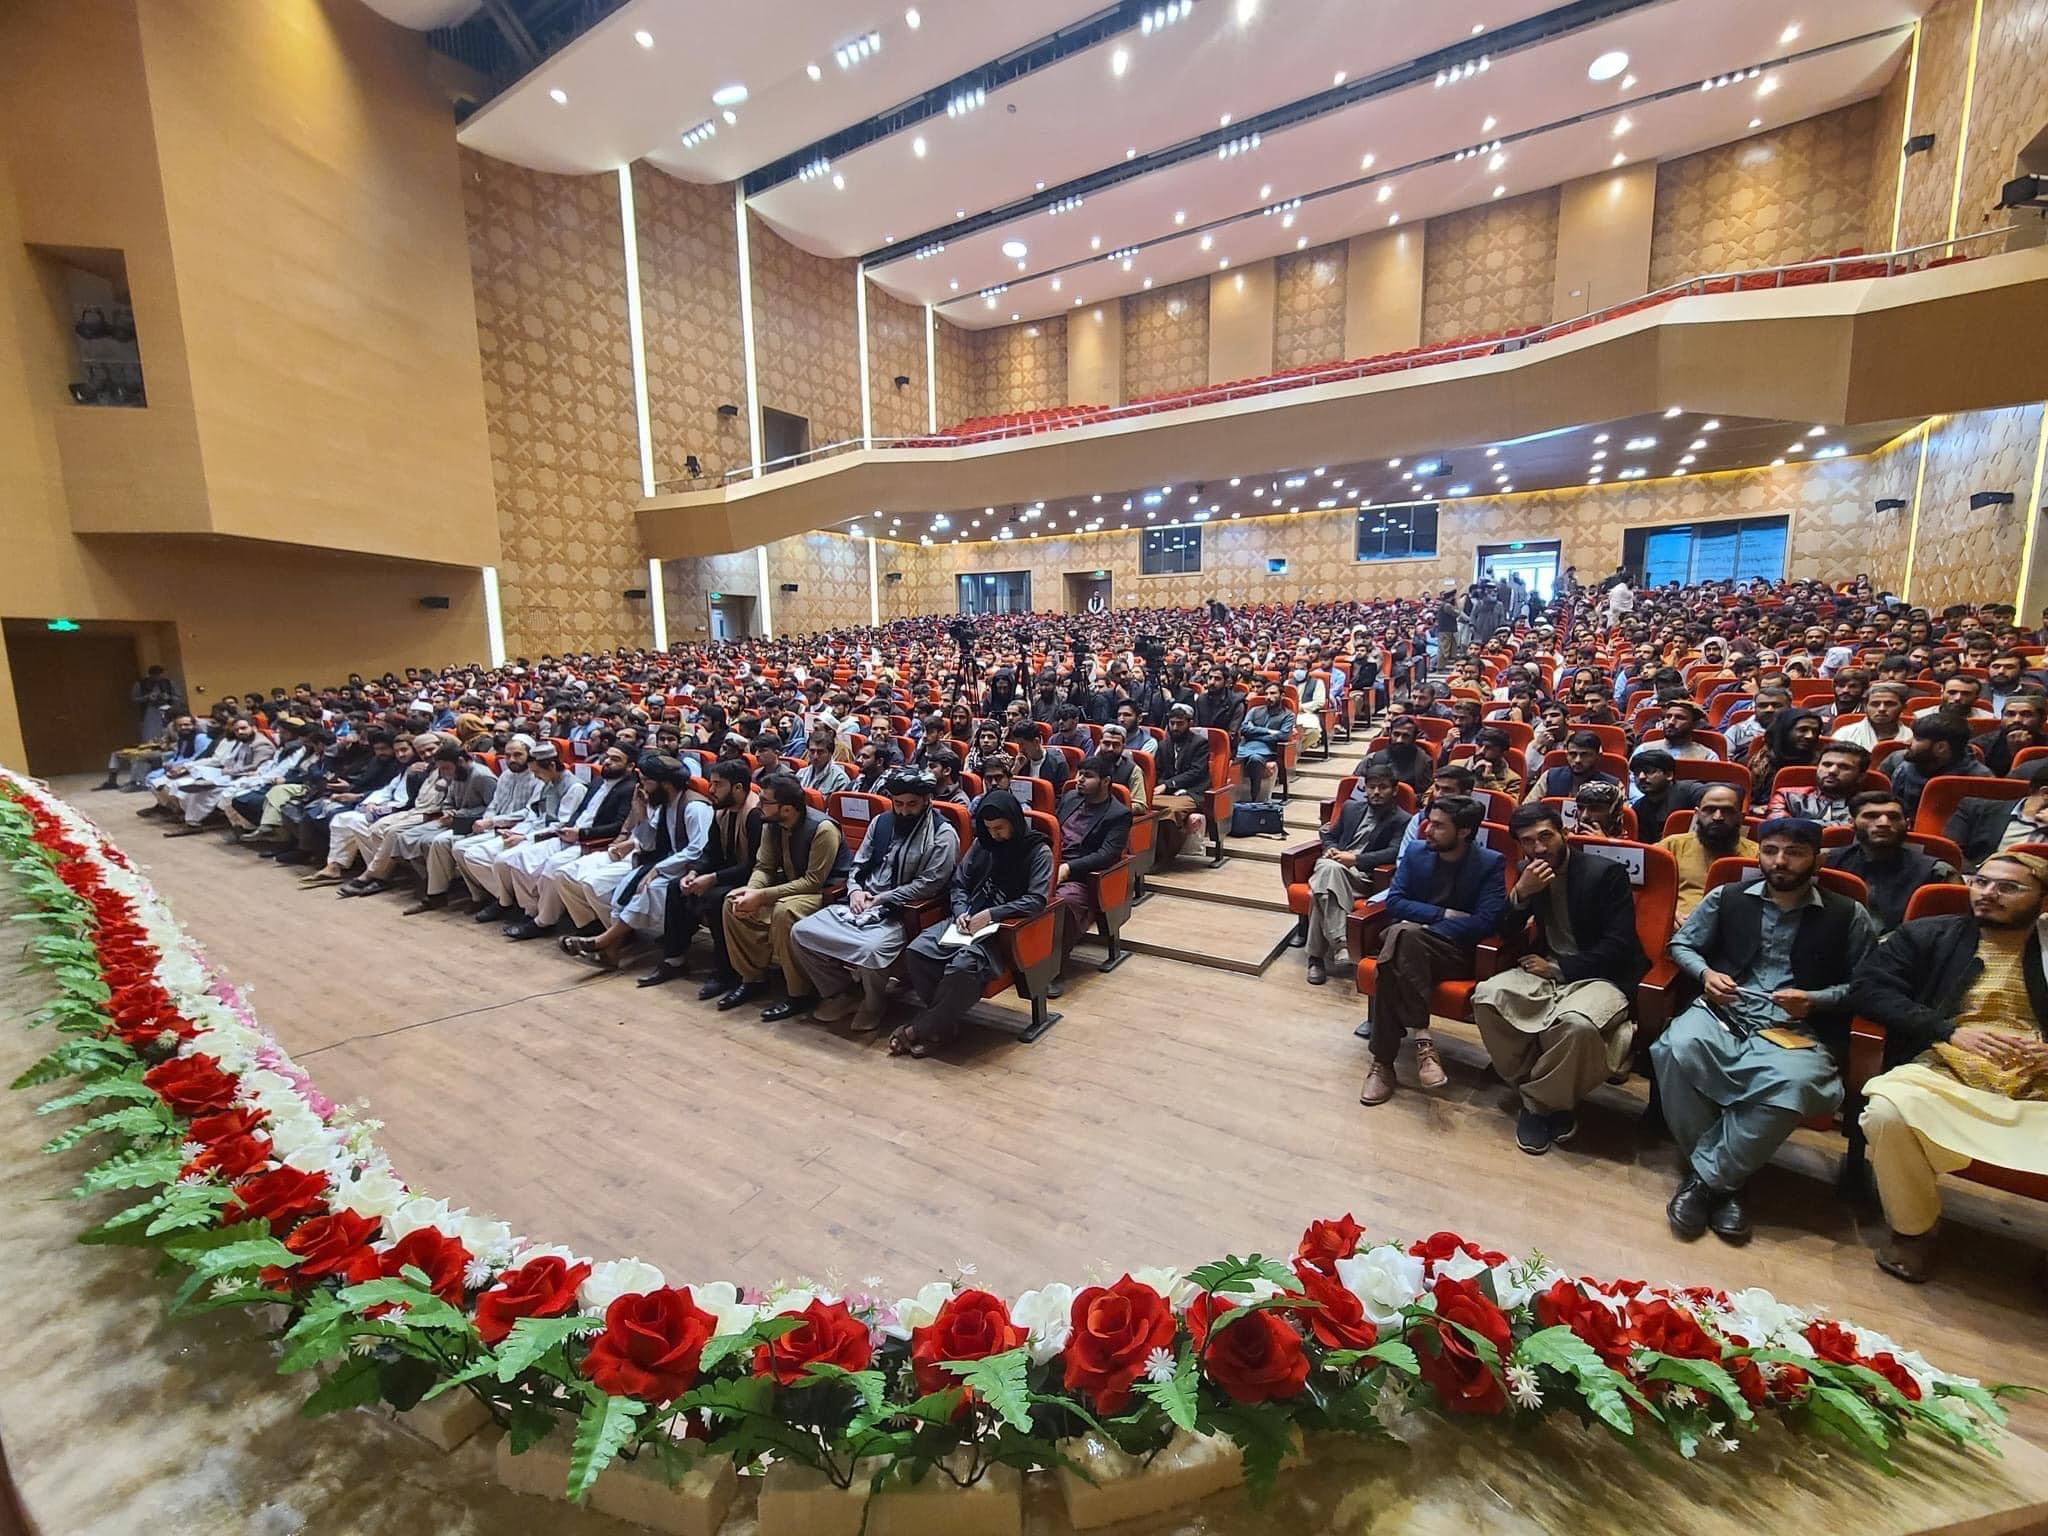
\includegraphics[width=1.0\textwidth]{Resources/KU2}
\caption{Kabul University}
\label{Figure:Kabul University}
\end{center}
\end{figure}

% ***************************************************

%CHAPTER 3
\chapter[Methodology]{Methodology}
\label{Chap:Methodology}


% ***************************************************
% Methodology
% ***************************************************

% ********* Enter your text below this line: ********

\section{Heading 1}
%Replace "Heading 1" with what will become the \label{} for this section.
\begin{itemize}
	\item Collecting materials, sources, information, studying, and providing information about writing notes
	
	\item Indicating the type and method of research
	\item	Demonstrate the effectiveness and benefits of the research method
	\item The relationship between the subject matter and the type and method of research
\end{itemize}
\subsection{Heading 2}
\lipsum[4] % This generates dummy text to fill the document



%CHAPTER 4
\chapter[Design]{Design}
\label{Chap:Design}


% ***************************************************
% Design
% ***************************************************

% ********* Enter your text below this line: ********

\section{Heading 1}
%Replace "Heading 1" with what will become the \label{} for this section.


\subsection{Heading 2}
\lipsum[4]

% ***************************************************

%CHAPTER 5
\chapter[Implementation]{Implementation}
\label{Chap:Implementation}


% ***************************************************
% Implementation
% ***************************************************

% ********* Enter your text below this line: ********
\section{Heading 1}
%Replace "Heading 1" with what will become the \label{} for this section.

\subsection{Heading 2}
\lipsum[4]

% ***************************************************

%CHAPTER 6
\input{./Chapter6/Results.tex}

%CHAPTER 6
\input{./Chapter7/Discussion.tex}


% HOW TO ADD ADDITIONAL CHAPTERS
% Step One: Add a new folder called "ChapterX" (X being the chapter number).
% Step Two: Within the folder add a new .tex file by clicking the "New File" button in the Overleaf Menu. Rename the file to a title of your choice.
% Step Three: Copy the Chapter 2 headline and "\input" command located above and insert it below Chapter 2.
% Step Four: Rename the headline to your specific chapter number, change the input command to include the name of the folder you created and the name of the file you created.
% Repeat this process for every chapter.

%CONCLUSION CHAPTER
% ***************************************************
% Conclusion
% ***************************************************
\chapter[Conclusion]{Conclusion}
\label{Chap:Conclusion}

% ********* Enter your text below this line: ********
\section{Conclusion}
\section{Limitation}
\section{Future Work}







% ***************************************************
% References
%****************************************************

%CHOOSE YOUR BIB STYLE AND FILE.
%We have included the following two referencing styles for you to use in your thesis. You can add an alternate style if you prefer.

%Style: apalike = this is an (Author, Year) referencing style similar to APA
%Style: elsarticle-num = this is a numbered referencing style that will display the bibliography in citation order

%To use one of the styles provided ensure the % is removed from the start of the line, and the other option is commented out with a % at the start of the line. The style elsarticle-num is active by default.

\bibliographystyle{apalike}
%\bibliographystyle{elsarticle-num}

\bibliography{./References/References}

\noindent \\
Use the referencing style appropriate to your \cite{Adachi2007} discipline refer to the \href{https://ku.edu.af}{\color{blue}{Kabul University}} for details.  

%When you have finished your thesis we recommend that you manually fix any errors in your bibliography. 
%To do this, compile, copy the .bbl into a new .tex file and include this here after commenting out the other bibliography commands. Make corrections in that .tex file.

% ***************************************************
% Appendices
%**************************************************** 

%UNCOMMENT THIS SECTION IF YOU ARE USING APPENDICES.
%Simply adapt the same formatting used for other chapters.
\appendix
% If you need appendix in your thesis then consider the following appendix file (you can add more if you need more) otherwise you should not consider it in your main thesis.
\include{./Appendix/Appendix}

\end{document}